\subsection{Проектирование и разработка базы данных}
\label{sec:design:database}

\subsubsection{} Разработка даталогической и физической моделей БД
\label{sec:design:database:model}

На даталогическом уровне модель предметной области представляется в привязке к конкретной СУБД и описывает способ организации данных безотносительно их физического размещения.
Описывать модель можно с помощью специальных графических нотаций~\cite{kulikov_db_workbook}.

В программном средстве, описываемом данным дипломным проектом, предполагается использование встроенной в платформу \andro СУБД \sqlite.
Из преимуществ данной СУБД стоит отметить следующие особенности:
\begin{itemize}
    \item Самодостаточность -- СУБД \sqlite не требуется отдельный сервер для работы.
    Она встраивается прямо в приложение и требует только доступ к файлам.
    Поэтому её возможно использовать локально без соединения с удаленным сервером.
    \item Высокая производительность – \sqlite потребляет мало ресурсов операционной системы и в силу отсутствия необходимости передачи данных по сети позволяет выполнять значительно быстрее по сравнению со стандартными серверными СУБД.
\end{itemize}

Однако, данная СУБД достаточно сильно ограничена типам данных, что стоит учитывать при разработке физической модели базы данных программного средства.
Типы данных, поддерживаемые СУБД \sqlite~\cite{sqlite_types}:
\begin{itemize}
    \item NULL -- пустое значение;
    \item INTEGER -- знаковое целое число, сохраненное в 1, 2, 3, 4, 6 или 8 байтах в зависимости от размера значения;
    \item REAL -- число с плавающей точкой, сохраненное в 8 байтах по стандарту IEEE-754~\cite{ieee_754};
    \item TEXT -- строковое значение, сохраненное в кодировке UTF-8;
    \item BLOB -- бинарные данные, сохраненные точно в том же виде.
\end{itemize}

В проектируемом программном средстве существует необходимость хранить данные некоторых типов, которые не поддерживаются этой СУБД, среди них временные значения и логические значения.

С учётом ограничений, временные значения предполагается хранить в текстовом виде с форматом записи по стандарту ISO~8601~\cite{iso_8601}.
Логические значения легко сохранять в качестве целочисленных значений 1 (Истина) и 0 (Ложь).

Также существует необходимость хранения нецелых денежных сумм, так как некоторые валюты могут состоять из дробных частей.
Для избежания погрешности в арифметических операциях с числами с плавающей точкой, предполагается хранение данных денежных сумм в текстовом виде с округлением до двух знаков после запятой.

Физическая модель базы данных представлена на рисунке~\ref{fig:design:database:model:diagram}.

Далее подробнее рассматривается некоторые особенности физической модели базы данных:
\begin{enumerate}
    \item Каждая сущность представлена своей таблицей.
    \item Все таблицы сущностей имеют поля, предназначенные для хранения глобального идентификатора (external\_id).
    По умолчанию эти поля имеют значение NULL, потому что новые данные, созданные локально, не могут иметь глобального идентификатора без успешной синхронизации.
    \item Журнал изменений, описанный в пункте~\ref{sec:design:sync} для каждой сущности представлен в виде отдельной таблицы, которая содержат в себе все поля, что и таблицы сущностей, но с некоторыми дополнительными атрибутами:
    \begin{enumerate}
        \item Поле action\_id представляет собой уникальный идентификатор записи в журнале.
        \item Поле action\_type указывает на то, какой тип операции был произведен над сущностью.
        Предполагается, что поле может содержать одно из значений <<INSERT>>, <<UPDATE>> и <<DELETE>>.
        \item Поле action\_timestamp отображает время совершения операции для последующего определения приоритета в конфликтных ситуациях.
    \end{enumerate}
    \item Параметры отображения сущности <<Валюта>> в физической модели базы данных представлены двумя атрибутами:
    \begin{enumerate}
        \item Поле symbol -- строковое значение, содержащее в себе знак валюты или общепринятую подпись денежных значений в данной валюте.
        Например, для валюты <<Белорусский рубль>> данное поле будет содержать значение <<руб.>>.
        \item Поле is\_prefix указывает на то, каким образом должна производиться запись подписи валюты и самого значения.
        При значении is\_prefix, равным единице, подпись валюты располагается до значения суммы.
    \end{enumerate}
    \item Атрибут <<Сумма перевода>> сущности <<Перевод между счетами>> в физической модели представлен двумя атрибутами, отображающими суммы переводов счёта-отправителя и счёта-получателя соответственно.
    Разделение данного атрибута необходимо для поддержки множественных валют, так как эти суммы могут не совпадать.
\end{enumerate}

\begin{figure}[p]
    \centering
    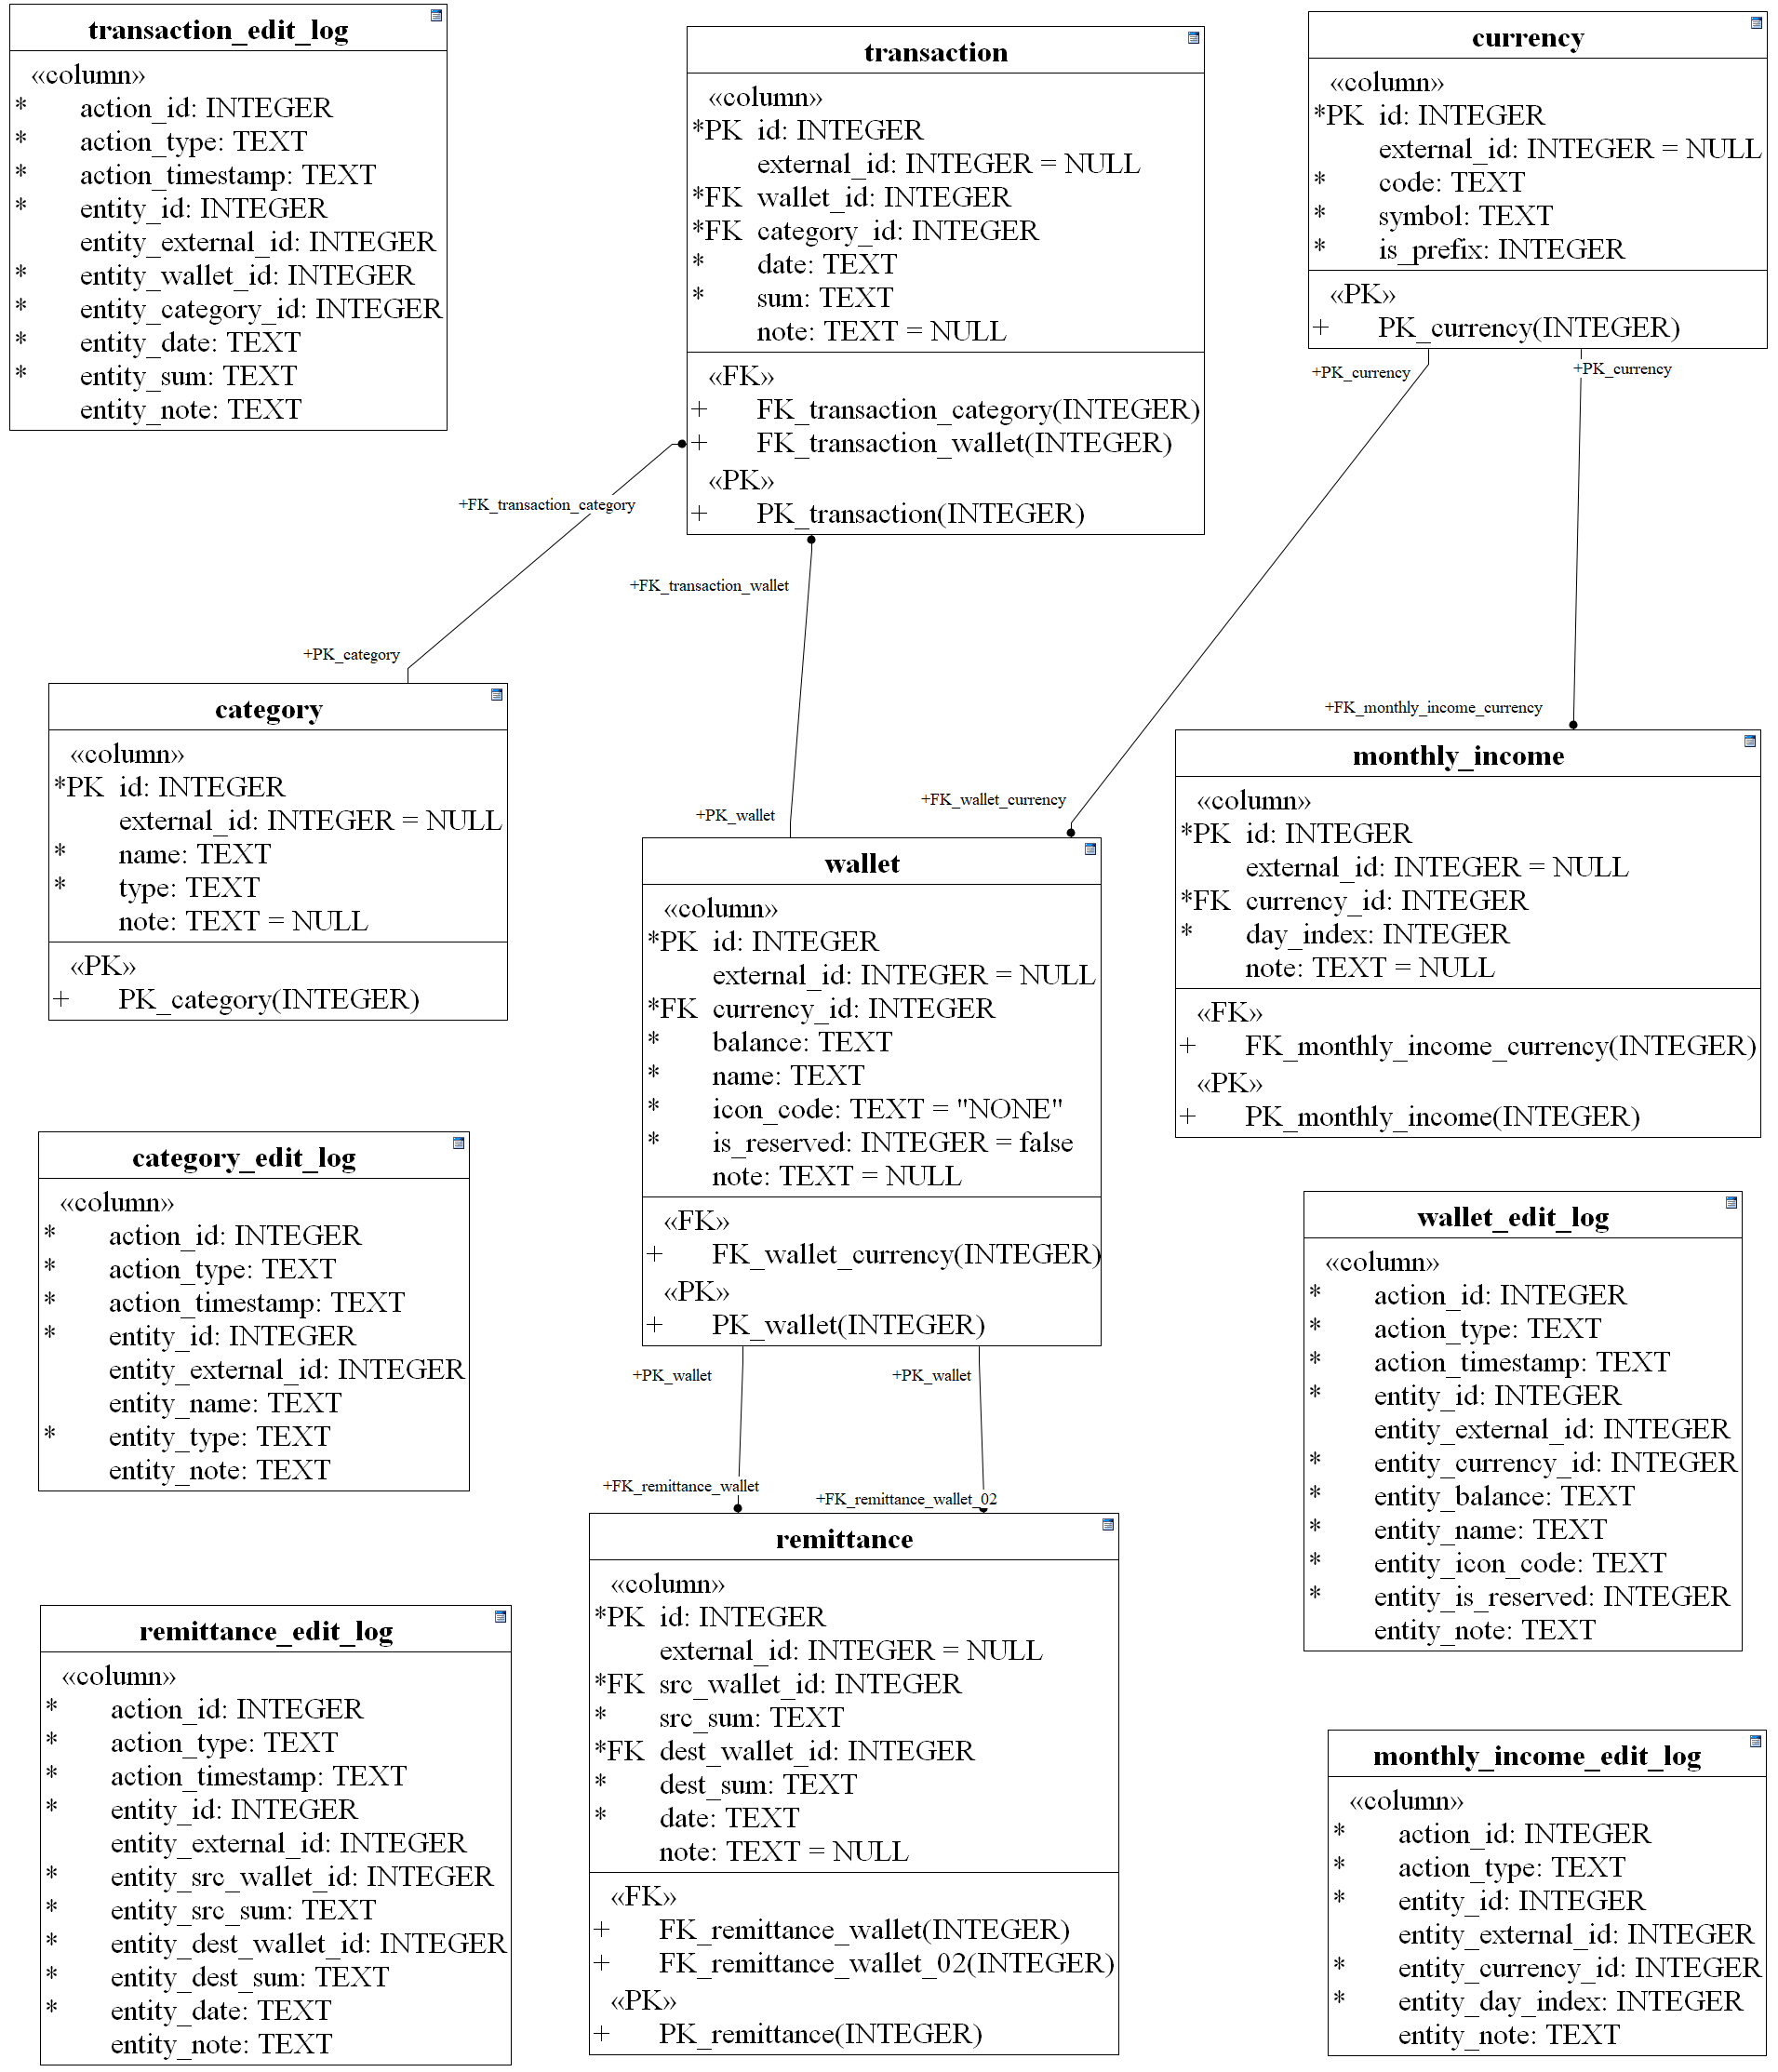
\includegraphics[scale=0.33]{3_4_physical_model.png}
    \caption{Физическая модель базы данных ПС}
    \label{fig:design:database:model:diagram}
\end{figure}

Регистрация операций с сущностями в таблицах журналов изменений можно реализовать при помощи встроенных в СУБД \sqlite триггеров -- хранимых процедур особого типа, исполнение которых обусловлено действием по модификации данных над определённой таблицей базы данных.
Таким образом, при проведении операции с какой-либо таблицей сущности, изменения будут автоматически записываться в соответствующую таблицу журнала изменений.

\subsubsection{} Организация доступа к базе данных
\label{sec:design:database:implementation}

Для организации доступа к встроенной базе данных SQLite, в \andro SDK предусмотрен набор классов из пакета <<android.database.sqlite>>~\cite{android_sqlite}.
Данный набор классов предоставляет широкий спектр возможностей по манипуляции с базой данных, однако имеет некоторые недостатки:
\begin{itemize}
    \item отсутствие проверки SQL-запросов во время компиляции;
    \item при изменении схемы данных требуется вручную обновлять затронутые SQL-запросы, этот процесс может быть длительным и подверженным ошибкам;
    \item надо писать сравнительно большое шаблонного кода для конвертации между SQL и Kotlin-объектами модели данных.
\end{itemize}

Компания Google, которая также занимается разработкой операционной системы \andro, в 2017 году представила набор библиотек Android Architecture Com\-po\-nents~\cite{android_components}, которые призваны упростить и улучшить некоторые стандартные аспекты разработки для платформы Android.
Один из таких компонентов, библиотека Room, предоставляет слой отображения  объектов (object-mapping abstraction layer), позволяющий организовать простой доступ к базе данных наряду со всей мощью \sqlite.
Библиотека Room помогает избавиться от всех описанных выше недостатков использования стандартных средств по работе с БД.

Room имеет три основных компонента:
\begin{itemize}
    \item Entity -- класс, который представляет собой проекцию таблицы СУБД \sqlite в коде приложения.
    \item DAO -- интерфейс, в котором содержатся методы по непосредственному взаимодействию с данными.
    На этапе компиляции библиотекой будет сгенерирована реализация данного класса, содержащая весь низкоуровневый код по работе с \sqlite.
    \item Database -- класс, отвечающий за доступ к базе данных в коде приложения.
\end{itemize}

Из описанного выше следует, что для организации доступа к базе данных, требуется реализовать классы DAO и Entity для каждой из описанных сущностей программного средства, а также единственный объект Database для доступа к ним.
Для предоставления библиотеке Room информации о разрабатываемой базе данных необходимо описать классы необходимыми аннотациями -- специальной формой синтаксических метаданных, которая может быть добавлена в исходный код для компилятора или интерпретатора языка.

Процесс описания сущности <<Категория>> (Category) при помощи библиотеки Room:

\begin{lstlisting}[style=standard]
// `Определение класса как таблицы базы данных с именем tableName`
@Entity(tableName = "category")
// `Указание классов-преобразователей для типов данный, которые неизвестны`
// `для библиотеки Room`
@TypeConverters(CategoryConverters::class)
data class RoomCategory(
    // `Определение поля id как первичного ключа в таблице`
    @PrimaryKey(autoGenerate = true)
    @ColumnInfo(name = "id")
    // `Уникальный локальный идентификатор категории`
    var id: Long,
    // `Указание другого типа имени в самой базе данных для соответствия схеме`
    @ColumnInfo(name = "external_id")
    // `Глобальный идентификатор категории`
    var externalId: Long?,
    @ColumnInfo(name = "type")
    // `Тип категории (доход или расход)`
    var type: CategoryType,
    @ColumnInfo(name = "name")
    // `Имя категории`
    var name: String,
    @ColumnInfo(name = "note")
    // `Необязательное описание категории`
    var note: String?
)
\end{lstlisting}

Аналогичным образом требуется описать все сущности разрабатываемой базы данных.

По умолчанию библиотека Room может конвертировать большое множество стандартных типов данных языка Java (и \kt в силу его полной совместимости с языком Java) в типы данных СУБД \sqlite.
Однако бывают такие ситуации, когда требуется преобразовывать собственный тип данных в один из типов \sqlite, например тип CategoryType:
\begin{lstlisting}[style=standard]
// `Перечисление типов пользовательской категории`
enum class CategoryType {
    // `Транзакции с категорией такого типа определяются как доход`
    INCOME,
    // `Транзакции с категорией такого типа определяются как расход`
    EXPENSE
}
\end{lstlisting}

Для решения данной проблемы библиотека предоставляет возможность определения своих классов-преобразователей.
Библиотека определяет такие классы при помощи аннотации @TypeConverters над классом таблицы.
Далее библиотека определяет все методы с аннотацией @TypeConverter и типы возвращаемого и принимаемого значений каждого метода:
\begin{lstlisting}[style=standard]
// `Класс-преобразователь для неизвестных типов таблицы категорий`
class CategoryConverters {
    // `Определение метода как преобразующего`
    @TypeConverter
    // `Преобразует тип String в CategoryType для получения данных из базы`
    fun categoryTypeFromString(value: String?): CategoryType? =
            value?.let { CategoryType.valueOf(value) }
    @TypeConverter
    // `Преобразует тип CategoryType в String для сохранения данных в базу`
    fun stringFromCategoryType(value: CategoryType?): String? = value?.name
}
\end{lstlisting}

Чтобы предоставить доступ к базе данных для предметной области приложения, как описано в пункте~\ref{sec:design:business}, требуется реализовать интерфейс соответствующие интерфейсы Storage, StorageTransactionManager, а также методы конвертации объектов Room в сущности предметной области.